%%%%%%%%%%%%%%%%%%%%%%%%%%%%%% -*- Mode: Latex -*- %%%%%%%%%%%%%%%%%%%%%%%%%%%%
%% 04-22.tex -- P-PHEC Workshop Paper on HackyHPC
%% Author          : Philip Johnson, Mike Paulding
%% Created On      : Wed Dec 08 2004
%% Last Modified By: Philip M. Johnson
%% Last Modified On: Mon Jan 24 10:11:59 2005
%% RCS: $Id$
%%%%%%%%%%%%%%%%%%%%%%%%%%%%%%%%%%%%%%%%%%%%%%%%%%%%%%%%%%%%%%%%%%%%%%%%%%%%%%%
%%   Copyright (C) 2002 Philip Johnson
%%%%%%%%%%%%%%%%%%%%%%%%%%%%%%%%%%%%%%%%%%%%%%%%%%%%%%%%%%%%%%%%%%%%%%%%%%%%%%%
%% 

\documentclass[10pt,twocolumn]{article} 
% Psfig/TeX 
\def\PsfigVersion{1.9}
% dvips version
%
% All psfig/tex software, documentation, and related files
% in this distribution of psfig/tex are 
% Copyright 1987, 1988, 1991 Trevor J. Darrell
%
% Permission is granted for use and non-profit distribution of psfig/tex 
% providing that this notice is clearly maintained. The right to
% distribute any portion of psfig/tex for profit or as part of any commercial
% product is specifically reserved for the author(s) of that portion.
%
% *** Feel free to make local modifications of psfig as you wish,
% *** but DO NOT post any changed or modified versions of ``psfig''
% *** directly to the net. Send them to me and I'll try to incorporate
% *** them into future versions. If you want to take the psfig code 
% *** and make a new program (subject to the copyright above), distribute it, 
% *** (and maintain it) that's fine, just don't call it psfig.
%
% Bugs and improvements to trevor@media.mit.edu.
%
% Thanks to Greg Hager (GDH) and Ned Batchelder for their contributions
% to the original version of this project.
%
% Modified by J. Daniel Smith on 9 October 1990 to accept the
% %%BoundingBox: comment with or without a space after the colon.  Stole
% file reading code from Tom Rokicki's EPSF.TEX file (see below).
%
% More modifications by J. Daniel Smith on 29 March 1991 to allow the
% the included PostScript figure to be rotated.  The amount of
% rotation is specified by the "angle=" parameter of the \psfig command.
%
% Modified by Robert Russell on June 25, 1991 to allow users to specify
% .ps filenames which don't yet exist, provided they explicitly provide
% boundingbox information via the \psfig command. Note: This will only work
% if the "file=" parameter follows all four "bb???=" parameters in the
% command. This is due to the order in which psfig interprets these params.
%
%  3 Jul 1991	JDS	check if file already read in once
%  4 Sep 1991	JDS	fixed incorrect computation of rotated
%			bounding box
% 25 Sep 1991	GVR	expanded synopsis of \psfig
% 14 Oct 1991	JDS	\fbox code from LaTeX so \psdraft works with TeX
%			changed \typeout to \ps@typeout
% 17 Oct 1991	JDS	added \psscalefirst and \psrotatefirst
%

% From: gvr@cs.brown.edu (George V. Reilly)
%
% \psdraft	draws an outline box, but doesn't include the figure
%		in the DVI file.  Useful for previewing.
%
% \psfull	includes the figure in the DVI file (default).
%
% \psscalefirst width= or height= specifies the size of the figure
% 		before rotation.
% \psrotatefirst (default) width= or height= specifies the size of the
% 		 figure after rotation.  Asymetric figures will
% 		 appear to shrink.
%
% \psfigurepath#1	sets the path to search for the figure
%
% \psfig
% usage: \psfig{file=, figure=, height=, width=,
%			bbllx=, bblly=, bburx=, bbury=,
%			rheight=, rwidth=, clip=, angle=, silent=}
%
%	"file" is the filename.  If no path name is specified and the
%		file is not found in the current directory,
%		it will be looked for in directory \psfigurepath.
%	"figure" is a synonym for "file".
%	By default, the width and height of the figure are taken from
%		the BoundingBox of the figure.
%	If "width" is specified, the figure is scaled so that it has
%		the specified width.  Its height changes proportionately.
%	If "height" is specified, the figure is scaled so that it has
%		the specified height.  Its width changes proportionately.
%	If both "width" and "height" are specified, the figure is scaled
%		anamorphically.
%	"bbllx", "bblly", "bburx", and "bbury" control the PostScript
%		BoundingBox.  If these four values are specified
%               *before* the "file" option, the PSFIG will not try to
%               open the PostScript file.
%	"rheight" and "rwidth" are the reserved height and width
%		of the figure, i.e., how big TeX actually thinks
%		the figure is.  They default to "width" and "height".
%	The "clip" option ensures that no portion of the figure will
%		appear outside its BoundingBox.  "clip=" is a switch and
%		takes no value, but the `=' must be present.
%	The "angle" option specifies the angle of rotation (degrees, ccw).
%	The "silent" option makes \psfig work silently.
%

% check to see if macros already loaded in (maybe some other file says
% "\input psfig") ...
\ifx\undefined\psfig\else\endinput\fi

%
% from a suggestion by eijkhout@csrd.uiuc.edu to allow
% loading as a style file. Changed to avoid problems
% with amstex per suggestion by jbence@math.ucla.edu

\let\LaTeXAtSign=\@
\let\@=\relax
\edef\psfigRestoreAt{\catcode`\@=\number\catcode`@\relax}
%\edef\psfigRestoreAt{\catcode`@=\number\catcode`@\relax}
\catcode`\@=11\relax
\newwrite\@unused
\def\ps@typeout#1{{\let\protect\string\immediate\write\@unused{#1}}}
\ps@typeout{psfig/tex \PsfigVersion}

%% Here's how you define your figure path.  Should be set up with null
%% default and a user useable definition.

\def\figurepath{./}
\def\psfigurepath#1{\edef\figurepath{#1}}

%
% @psdo control structure -- similar to Latex @for.
% I redefined these with different names so that psfig can
% be used with TeX as well as LaTeX, and so that it will not 
% be vunerable to future changes in LaTeX's internal
% control structure,
%
\def\@nnil{\@nil}
\def\@empty{}
\def\@psdonoop#1\@@#2#3{}
\def\@psdo#1:=#2\do#3{\edef\@psdotmp{#2}\ifx\@psdotmp\@empty \else
    \expandafter\@psdoloop#2,\@nil,\@nil\@@#1{#3}\fi}
\def\@psdoloop#1,#2,#3\@@#4#5{\def#4{#1}\ifx #4\@nnil \else
       #5\def#4{#2}\ifx #4\@nnil \else#5\@ipsdoloop #3\@@#4{#5}\fi\fi}
\def\@ipsdoloop#1,#2\@@#3#4{\def#3{#1}\ifx #3\@nnil 
       \let\@nextwhile=\@psdonoop \else
      #4\relax\let\@nextwhile=\@ipsdoloop\fi\@nextwhile#2\@@#3{#4}}
\def\@tpsdo#1:=#2\do#3{\xdef\@psdotmp{#2}\ifx\@psdotmp\@empty \else
    \@tpsdoloop#2\@nil\@nil\@@#1{#3}\fi}
\def\@tpsdoloop#1#2\@@#3#4{\def#3{#1}\ifx #3\@nnil 
       \let\@nextwhile=\@psdonoop \else
      #4\relax\let\@nextwhile=\@tpsdoloop\fi\@nextwhile#2\@@#3{#4}}
% 
% \fbox is defined in latex.tex; so if \fbox is undefined, assume that
% we are not in LaTeX.
% Perhaps this could be done better???
\ifx\undefined\fbox
% \fbox code from modified slightly from LaTeX
\newdimen\fboxrule
\newdimen\fboxsep
\newdimen\ps@tempdima
\newbox\ps@tempboxa
\fboxsep = 3pt
\fboxrule = .4pt
\long\def\fbox#1{\leavevmode\setbox\ps@tempboxa\hbox{#1}\ps@tempdima\fboxrule
    \advance\ps@tempdima \fboxsep \advance\ps@tempdima \dp\ps@tempboxa
   \hbox{\lower \ps@tempdima\hbox
  {\vbox{\hrule height \fboxrule
          \hbox{\vrule width \fboxrule \hskip\fboxsep
          \vbox{\vskip\fboxsep \box\ps@tempboxa\vskip\fboxsep}\hskip 
                 \fboxsep\vrule width \fboxrule}
                 \hrule height \fboxrule}}}}
\fi
%
%%%%%%%%%%%%%%%%%%%%%%%%%%%%%%%%%%%%%%%%%%%%%%%%%%%%%%%%%%%%%%%%%%%
% file reading stuff from epsf.tex
%   EPSF.TEX macro file:
%   Written by Tomas Rokicki of Radical Eye Software, 29 Mar 1989.
%   Revised by Don Knuth, 3 Jan 1990.
%   Revised by Tomas Rokicki to accept bounding boxes with no
%      space after the colon, 18 Jul 1990.
%   Portions modified/removed for use in PSFIG package by
%      J. Daniel Smith, 9 October 1990.
%
\newread\ps@stream
\newif\ifnot@eof       % continue looking for the bounding box?
\newif\if@noisy        % report what you're making?
\newif\if@atend        % %%BoundingBox: has (at end) specification
\newif\if@psfile       % does this look like a PostScript file?
%
% PostScript files should start with `%!'
%
{\catcode`\%=12\global\gdef\epsf@start{%!}}
\def\epsf@PS{PS}
%
\def\epsf@getbb#1{%
%
%   The first thing we need to do is to open the
%   PostScript file, if possible.
%
\openin\ps@stream=#1
\ifeof\ps@stream\ps@typeout{Error, File #1 not found}\else
%
%   Okay, we got it. Now we'll scan lines until we find one that doesn't
%   start with %. We're looking for the bounding box comment.
%
   {\not@eoftrue \chardef\other=12
    \def\do##1{\catcode`##1=\other}\dospecials \catcode`\ =10
    \loop
       \if@psfile
	  \read\ps@stream to \epsf@fileline
       \else{
	  \obeyspaces
          \read\ps@stream to \epsf@tmp\global\let\epsf@fileline\epsf@tmp}
       \fi
       \ifeof\ps@stream\not@eoffalse\else
%
%   Check the first line for `%!'.  Issue a warning message if its not
%   there, since the file might not be a PostScript file.
%
       \if@psfile\else
       \expandafter\epsf@test\epsf@fileline:. \\%
       \fi
%
%   We check to see if the first character is a % sign;
%   if so, we look further and stop only if the line begins with
%   `%%BoundingBox:' and the `(atend)' specification was not found.
%   That is, the only way to stop is when the end of file is reached,
%   or a `%%BoundingBox: llx lly urx ury' line is found.
%
          \expandafter\epsf@aux\epsf@fileline:. \\%
       \fi
   \ifnot@eof\repeat
   }\closein\ps@stream\fi}%
%
% This tests if the file we are reading looks like a PostScript file.
%
\long\def\epsf@test#1#2#3:#4\\{\def\epsf@testit{#1#2}
			\ifx\epsf@testit\epsf@start\else
\ps@typeout{Warning! File does not start with `\epsf@start'.  It may not be a PostScript file.}
			\fi
			\@psfiletrue} % don't test after 1st line
%
%   We still need to define the tricky \epsf@aux macro. This requires
%   a couple of magic constants for comparison purposes.
%
{\catcode`\%=12\global\let\epsf@percent=%\global\def\epsf@bblit{%BoundingBox}}
%
%
%   So we're ready to check for `%BoundingBox:' and to grab the
%   values if they are found.  We continue searching if `(at end)'
%   was found after the `%BoundingBox:'.
%
\long\def\epsf@aux#1#2:#3\\{\ifx#1\epsf@percent
   \def\epsf@testit{#2}\ifx\epsf@testit\epsf@bblit
	\@atendfalse
        \epsf@atend #3 . \\%
	\if@atend	
	   \if@verbose{
		\ps@typeout{psfig: found `(atend)'; continuing search}
	   }\fi
        \else
        \epsf@grab #3 . . . \\%
        \not@eoffalse
        \global\no@bbfalse
        \fi
   \fi\fi}%
%
%   Here we grab the values and stuff them in the appropriate definitions.
%
\def\epsf@grab #1 #2 #3 #4 #5\\{%
   \global\def\epsf@llx{#1}\ifx\epsf@llx\empty
      \epsf@grab #2 #3 #4 #5 .\\\else
   \global\def\epsf@lly{#2}%
   \global\def\epsf@urx{#3}\global\def\epsf@ury{#4}\fi}%
%
% Determine if the stuff following the %%BoundingBox is `(atend)'
% J. Daniel Smith.  Copied from \epsf@grab above.
%
\def\epsf@atendlit{(atend)} 
\def\epsf@atend #1 #2 #3\\{%
   \def\epsf@tmp{#1}\ifx\epsf@tmp\empty
      \epsf@atend #2 #3 .\\\else
   \ifx\epsf@tmp\epsf@atendlit\@atendtrue\fi\fi}


% End of file reading stuff from epsf.tex
%%%%%%%%%%%%%%%%%%%%%%%%%%%%%%%%%%%%%%%%%%%%%%%%%%%%%%%%%%%%%%%%%%%

%%%%%%%%%%%%%%%%%%%%%%%%%%%%%%%%%%%%%%%%%%%%%%%%%%%%%%%%%%%%%%%%%%%
% trigonometry stuff from "trig.tex"
\chardef\psletter = 11 % won't conflict with \begin{letter} now...
\chardef\other = 12

\newif \ifdebug %%% turn me on to see TeX hard at work ...
\newif\ifc@mpute %%% don't need to compute some values
\c@mputetrue % but assume that we do

\let\then = \relax
\def\r@dian{pt }
\let\r@dians = \r@dian
\let\dimensionless@nit = \r@dian
\let\dimensionless@nits = \dimensionless@nit
\def\internal@nit{sp }
\let\internal@nits = \internal@nit
\newif\ifstillc@nverging
\def \Mess@ge #1{\ifdebug \then \message {#1} \fi}

{ %%% Things that need abnormal catcodes %%%
	\catcode `\@ = \psletter
	\gdef \nodimen {\expandafter \n@dimen \the \dimen}
	\gdef \term #1 #2 #3%
	       {\edef \t@ {\the #1}%%% freeze parameter 1 (count, by value)
		\edef \t@@ {\expandafter \n@dimen \the #2\r@dian}%
				   %%% freeze parameter 2 (dimen, by value)
		\t@rm {\t@} {\t@@} {#3}%
	       }
	\gdef \t@rm #1 #2 #3%
	       {{%
		\count 0 = 0
		\dimen 0 = 1 \dimensionless@nit
		\dimen 2 = #2\relax
		\Mess@ge {Calculating term #1 of \nodimen 2}%
		\loop
		\ifnum	\count 0 < #1
		\then	\advance \count 0 by 1
			\Mess@ge {Iteration \the \count 0 \space}%
			\Multiply \dimen 0 by {\dimen 2}%
			\Mess@ge {After multiplication, term = \nodimen 0}%
			\Divide \dimen 0 by {\count 0}%
			\Mess@ge {After division, term = \nodimen 0}%
		\repeat
		\Mess@ge {Final value for term #1 of 
				\nodimen 2 \space is \nodimen 0}%
		\xdef \Term {#3 = \nodimen 0 \r@dians}%
		\aftergroup \Term
	       }}
	\catcode `\p = \other
	\catcode `\t = \other
	\gdef \n@dimen #1pt{#1} %%% throw away the ``pt''
}

\def \Divide #1by #2{\divide #1 by #2} %%% just a synonym

\def \Multiply #1by #2%%% allows division of a dimen by a dimen
       {{%%% should really freeze parameter 2 (dimen, passed by value)
	\count 0 = #1\relax
	\count 2 = #2\relax
	\count 4 = 65536
	\Mess@ge {Before scaling, count 0 = \the \count 0 \space and
			count 2 = \the \count 2}%
	\ifnum	\count 0 > 32767 %%% do our best to avoid overflow
	\then	\divide \count 0 by 4
		\divide \count 4 by 4
	\else	\ifnum	\count 0 < -32767
		\then	\divide \count 0 by 4
			\divide \count 4 by 4
		\else
		\fi
	\fi
	\ifnum	\count 2 > 32767 %%% while retaining reasonable accuracy
	\then	\divide \count 2 by 4
		\divide \count 4 by 4
	\else	\ifnum	\count 2 < -32767
		\then	\divide \count 2 by 4
			\divide \count 4 by 4
		\else
		\fi
	\fi
	\multiply \count 0 by \count 2
	\divide \count 0 by \count 4
	\xdef \product {#1 = \the \count 0 \internal@nits}%
	\aftergroup \product
       }}

\def\r@duce{\ifdim\dimen0 > 90\r@dian \then   % sin(x+90) = sin(180-x)
		\multiply\dimen0 by -1
		\advance\dimen0 by 180\r@dian
		\r@duce
	    \else \ifdim\dimen0 < -90\r@dian \then  % sin(-x) = sin(360+x)
		\advance\dimen0 by 360\r@dian
		\r@duce
		\fi
	    \fi}

\def\Sine#1%
       {{%
	\dimen 0 = #1 \r@dian
	\r@duce
	\ifdim\dimen0 = -90\r@dian \then
	   \dimen4 = -1\r@dian
	   \c@mputefalse
	\fi
	\ifdim\dimen0 = 90\r@dian \then
	   \dimen4 = 1\r@dian
	   \c@mputefalse
	\fi
	\ifdim\dimen0 = 0\r@dian \then
	   \dimen4 = 0\r@dian
	   \c@mputefalse
	\fi
%
	\ifc@mpute \then
        	% convert degrees to radians
		\divide\dimen0 by 180
		\dimen0=3.141592654\dimen0
%
		\dimen 2 = 3.1415926535897963\r@dian %%% a well-known constant
		\divide\dimen 2 by 2 %%% we only deal with -pi/2 : pi/2
		\Mess@ge {Sin: calculating Sin of \nodimen 0}%
		\count 0 = 1 %%% see power-series expansion for sine
		\dimen 2 = 1 \r@dian %%% ditto
		\dimen 4 = 0 \r@dian %%% ditto
		\loop
			\ifnum	\dimen 2 = 0 %%% then we've done
			\then	\stillc@nvergingfalse 
			\else	\stillc@nvergingtrue
			\fi
			\ifstillc@nverging %%% then calculate next term
			\then	\term {\count 0} {\dimen 0} {\dimen 2}%
				\advance \count 0 by 2
				\count 2 = \count 0
				\divide \count 2 by 2
				\ifodd	\count 2 %%% signs alternate
				\then	\advance \dimen 4 by \dimen 2
				\else	\advance \dimen 4 by -\dimen 2
				\fi
		\repeat
	\fi		
			\xdef \sine {\nodimen 4}%
       }}

% Now the Cosine can be calculated easily by calling \Sine
\def\Cosine#1{\ifx\sine\UnDefined\edef\Savesine{\relax}\else
		             \edef\Savesine{\sine}\fi
	{\dimen0=#1\r@dian\advance\dimen0 by 90\r@dian
	 \Sine{\nodimen 0}
	 \xdef\cosine{\sine}
	 \xdef\sine{\Savesine}}}	      
% end of trig stuff
%%%%%%%%%%%%%%%%%%%%%%%%%%%%%%%%%%%%%%%%%%%%%%%%%%%%%%%%%%%%%%%%%%%%

\def\psdraft{
	\def\@psdraft{0}
	%\ps@typeout{draft level now is \@psdraft \space . }
}
\def\psfull{
	\def\@psdraft{100}
	%\ps@typeout{draft level now is \@psdraft \space . }
}

\psfull

\newif\if@scalefirst
\def\psscalefirst{\@scalefirsttrue}
\def\psrotatefirst{\@scalefirstfalse}
\psrotatefirst

\newif\if@draftbox
\def\psnodraftbox{
	\@draftboxfalse
}
\def\psdraftbox{
	\@draftboxtrue
}
\@draftboxtrue

\newif\if@prologfile
\newif\if@postlogfile
\def\pssilent{
	\@noisyfalse
}
\def\psnoisy{
	\@noisytrue
}
\psnoisy
%%% These are for the option list.
%%% A specification of the form a = b maps to calling \@p@@sa{b}
\newif\if@bbllx
\newif\if@bblly
\newif\if@bburx
\newif\if@bbury
\newif\if@height
\newif\if@width
\newif\if@rheight
\newif\if@rwidth
\newif\if@angle
\newif\if@clip
\newif\if@verbose
\def\@p@@sclip#1{\@cliptrue}


\newif\if@decmpr

%%% GDH 7/26/87 -- changed so that it first looks in the local directory,
%%% then in a specified global directory for the ps file.
%%% RPR 6/25/91 -- changed so that it defaults to user-supplied name if
%%% boundingbox info is specified, assuming graphic will be created by
%%% print time.
%%% TJD 10/19/91 -- added bbfile vs. file distinction, and @decmpr flag

\def\@p@@sfigure#1{\def\@p@sfile{null}\def\@p@sbbfile{null}
	        \openin1=#1.bb
		\ifeof1\closein1
	        	\openin1=\figurepath#1.bb
			\ifeof1\closein1
			        \openin1=#1
				\ifeof1\closein1%
				       \openin1=\figurepath#1
					\ifeof1
					   \ps@typeout{Error, File #1 not found}
						\if@bbllx\if@bblly
				   		\if@bburx\if@bbury
			      				\def\@p@sfile{#1}%
			      				\def\@p@sbbfile{#1}%
							\@decmprfalse
				  	   	\fi\fi\fi\fi
					\else\closein1
				    		\def\@p@sfile{\figurepath#1}%
				    		\def\@p@sbbfile{\figurepath#1}%
						\@decmprfalse
	                       		\fi%
			 	\else\closein1%
					\def\@p@sfile{#1}
					\def\@p@sbbfile{#1}
					\@decmprfalse
			 	\fi
			\else
				\def\@p@sfile{\figurepath#1}
				\def\@p@sbbfile{\figurepath#1.bb}
				\@decmprtrue
			\fi
		\else
			\def\@p@sfile{#1}
			\def\@p@sbbfile{#1.bb}
			\@decmprtrue
		\fi}

\def\@p@@sfile#1{\@p@@sfigure{#1}}

\def\@p@@sbbllx#1{
		%\ps@typeout{bbllx is #1}
		\@bbllxtrue
		\dimen100=#1
		\edef\@p@sbbllx{\number\dimen100}
}
\def\@p@@sbblly#1{
		%\ps@typeout{bblly is #1}
		\@bbllytrue
		\dimen100=#1
		\edef\@p@sbblly{\number\dimen100}
}
\def\@p@@sbburx#1{
		%\ps@typeout{bburx is #1}
		\@bburxtrue
		\dimen100=#1
		\edef\@p@sbburx{\number\dimen100}
}
\def\@p@@sbbury#1{
		%\ps@typeout{bbury is #1}
		\@bburytrue
		\dimen100=#1
		\edef\@p@sbbury{\number\dimen100}
}
\def\@p@@sheight#1{
		\@heighttrue
		\dimen100=#1
   		\edef\@p@sheight{\number\dimen100}
		%\ps@typeout{Height is \@p@sheight}
}
\def\@p@@swidth#1{
		%\ps@typeout{Width is #1}
		\@widthtrue
		\dimen100=#1
		\edef\@p@swidth{\number\dimen100}
}
\def\@p@@srheight#1{
		%\ps@typeout{Reserved height is #1}
		\@rheighttrue
		\dimen100=#1
		\edef\@p@srheight{\number\dimen100}
}
\def\@p@@srwidth#1{
		%\ps@typeout{Reserved width is #1}
		\@rwidthtrue
		\dimen100=#1
		\edef\@p@srwidth{\number\dimen100}
}
\def\@p@@sangle#1{
		%\ps@typeout{Rotation is #1}
		\@angletrue
%		\dimen100=#1
		\edef\@p@sangle{#1} %\number\dimen100}
}
\def\@p@@ssilent#1{ 
		\@verbosefalse
}
\def\@p@@sprolog#1{\@prologfiletrue\def\@prologfileval{#1}}
\def\@p@@spostlog#1{\@postlogfiletrue\def\@postlogfileval{#1}}
\def\@cs@name#1{\csname #1\endcsname}
\def\@setparms#1=#2,{\@cs@name{@p@@s#1}{#2}}
%
% initialize the defaults (size the size of the figure)
%
\def\ps@init@parms{
		\@bbllxfalse \@bbllyfalse
		\@bburxfalse \@bburyfalse
		\@heightfalse \@widthfalse
		\@rheightfalse \@rwidthfalse
		\def\@p@sbbllx{}\def\@p@sbblly{}
		\def\@p@sbburx{}\def\@p@sbbury{}
		\def\@p@sheight{}\def\@p@swidth{}
		\def\@p@srheight{}\def\@p@srwidth{}
		\def\@p@sangle{0}
		\def\@p@sfile{} \def\@p@sbbfile{}
		\def\@p@scost{10}
		\def\@sc{}
		\@prologfilefalse
		\@postlogfilefalse
		\@clipfalse
		\if@noisy
			\@verbosetrue
		\else
			\@verbosefalse
		\fi
}
%
% Go through the options setting things up.
%
\def\parse@ps@parms#1{
	 	\@psdo\@psfiga:=#1\do
		   {\expandafter\@setparms\@psfiga,}}
%
% Compute bb height and width
%
\newif\ifno@bb
\def\bb@missing{
	\if@verbose{
		\ps@typeout{psfig: searching \@p@sbbfile \space  for bounding box}
	}\fi
	\no@bbtrue
	\epsf@getbb{\@p@sbbfile}
        \ifno@bb \else \bb@cull\epsf@llx\epsf@lly\epsf@urx\epsf@ury\fi
}	
\def\bb@cull#1#2#3#4{
	\dimen100=#1 bp\edef\@p@sbbllx{\number\dimen100}
	\dimen100=#2 bp\edef\@p@sbblly{\number\dimen100}
	\dimen100=#3 bp\edef\@p@sbburx{\number\dimen100}
	\dimen100=#4 bp\edef\@p@sbbury{\number\dimen100}
	\no@bbfalse
}
% rotate point (#1,#2) about (0,0).
% The sine and cosine of the angle are already stored in \sine and
% \cosine.  The result is placed in (\p@intvaluex, \p@intvaluey).
\newdimen\p@intvaluex
\newdimen\p@intvaluey
\def\rotate@#1#2{{\dimen0=#1 sp\dimen1=#2 sp
%            	calculate x' = x \cos\theta - y \sin\theta
		  \global\p@intvaluex=\cosine\dimen0
		  \dimen3=\sine\dimen1
		  \global\advance\p@intvaluex by -\dimen3
% 		calculate y' = x \sin\theta + y \cos\theta
		  \global\p@intvaluey=\sine\dimen0
		  \dimen3=\cosine\dimen1
		  \global\advance\p@intvaluey by \dimen3
		  }}
\def\compute@bb{
		\no@bbfalse
		\if@bbllx \else \no@bbtrue \fi
		\if@bblly \else \no@bbtrue \fi
		\if@bburx \else \no@bbtrue \fi
		\if@bbury \else \no@bbtrue \fi
		\ifno@bb \bb@missing \fi
		\ifno@bb \ps@typeout{FATAL ERROR: no bb supplied or found}
			\no-bb-error
		\fi
		%
%\ps@typeout{BB: \@p@sbbllx, \@p@sbblly, \@p@sbburx, \@p@sbbury} 
%
% store height/width of original (unrotated) bounding box
		\count203=\@p@sbburx
		\count204=\@p@sbbury
		\advance\count203 by -\@p@sbbllx
		\advance\count204 by -\@p@sbblly
		\edef\ps@bbw{\number\count203}
		\edef\ps@bbh{\number\count204}
		%\ps@typeout{ psbbh = \ps@bbh, psbbw = \ps@bbw }
		\if@angle 
			\Sine{\@p@sangle}\Cosine{\@p@sangle}
	        	{\dimen100=\maxdimen\xdef\r@p@sbbllx{\number\dimen100}
					    \xdef\r@p@sbblly{\number\dimen100}
			                    \xdef\r@p@sbburx{-\number\dimen100}
					    \xdef\r@p@sbbury{-\number\dimen100}}
%
% Need to rotate all four points and take the X-Y extremes of the new
% points as the new bounding box.
                        \def\minmaxtest{
			   \ifnum\number\p@intvaluex<\r@p@sbbllx
			      \xdef\r@p@sbbllx{\number\p@intvaluex}\fi
			   \ifnum\number\p@intvaluex>\r@p@sbburx
			      \xdef\r@p@sbburx{\number\p@intvaluex}\fi
			   \ifnum\number\p@intvaluey<\r@p@sbblly
			      \xdef\r@p@sbblly{\number\p@intvaluey}\fi
			   \ifnum\number\p@intvaluey>\r@p@sbbury
			      \xdef\r@p@sbbury{\number\p@intvaluey}\fi
			   }
%			lower left
			\rotate@{\@p@sbbllx}{\@p@sbblly}
			\minmaxtest
%			upper left
			\rotate@{\@p@sbbllx}{\@p@sbbury}
			\minmaxtest
%			lower right
			\rotate@{\@p@sbburx}{\@p@sbblly}
			\minmaxtest
%			upper right
			\rotate@{\@p@sbburx}{\@p@sbbury}
			\minmaxtest
			\edef\@p@sbbllx{\r@p@sbbllx}\edef\@p@sbblly{\r@p@sbblly}
			\edef\@p@sbburx{\r@p@sbburx}\edef\@p@sbbury{\r@p@sbbury}
%\ps@typeout{rotated BB: \r@p@sbbllx, \r@p@sbblly, \r@p@sbburx, \r@p@sbbury}
		\fi
		\count203=\@p@sbburx
		\count204=\@p@sbbury
		\advance\count203 by -\@p@sbbllx
		\advance\count204 by -\@p@sbblly
		\edef\@bbw{\number\count203}
		\edef\@bbh{\number\count204}
		%\ps@typeout{ bbh = \@bbh, bbw = \@bbw }
}
%
% \in@hundreds performs #1 * (#2 / #3) correct to the hundreds,
%	then leaves the result in @result
%
\def\in@hundreds#1#2#3{\count240=#2 \count241=#3
		     \count100=\count240	% 100 is first digit #2/#3
		     \divide\count100 by \count241
		     \count101=\count100
		     \multiply\count101 by \count241
		     \advance\count240 by -\count101
		     \multiply\count240 by 10
		     \count101=\count240	%101 is second digit of #2/#3
		     \divide\count101 by \count241
		     \count102=\count101
		     \multiply\count102 by \count241
		     \advance\count240 by -\count102
		     \multiply\count240 by 10
		     \count102=\count240	% 102 is the third digit
		     \divide\count102 by \count241
		     \count200=#1\count205=0
		     \count201=\count200
			\multiply\count201 by \count100
		 	\advance\count205 by \count201
		     \count201=\count200
			\divide\count201 by 10
			\multiply\count201 by \count101
			\advance\count205 by \count201
			%
		     \count201=\count200
			\divide\count201 by 100
			\multiply\count201 by \count102
			\advance\count205 by \count201
			%
		     \edef\@result{\number\count205}
}
\def\compute@wfromh{
		% computing : width = height * (bbw / bbh)
		\in@hundreds{\@p@sheight}{\@bbw}{\@bbh}
		%\ps@typeout{ \@p@sheight * \@bbw / \@bbh, = \@result }
		\edef\@p@swidth{\@result}
		%\ps@typeout{w from h: width is \@p@swidth}
}
\def\compute@hfromw{
		% computing : height = width * (bbh / bbw)
	        \in@hundreds{\@p@swidth}{\@bbh}{\@bbw}
		%\ps@typeout{ \@p@swidth * \@bbh / \@bbw = \@result }
		\edef\@p@sheight{\@result}
		%\ps@typeout{h from w : height is \@p@sheight}
}
\def\compute@handw{
		\if@height 
			\if@width
			\else
				\compute@wfromh
			\fi
		\else 
			\if@width
				\compute@hfromw
			\else
				\edef\@p@sheight{\@bbh}
				\edef\@p@swidth{\@bbw}
			\fi
		\fi
}
\def\compute@resv{
		\if@rheight \else \edef\@p@srheight{\@p@sheight} \fi
		\if@rwidth \else \edef\@p@srwidth{\@p@swidth} \fi
		%\ps@typeout{rheight = \@p@srheight, rwidth = \@p@srwidth}
}
%		
% Compute any missing values
\def\compute@sizes{
	\compute@bb
	\if@scalefirst\if@angle
% at this point the bounding box has been adjsuted correctly for
% rotation.  PSFIG does all of its scaling using \@bbh and \@bbw.  If
% a width= or height= was specified along with \psscalefirst, then the
% width=/height= value needs to be adjusted to match the new (rotated)
% bounding box size (specifed in \@bbw and \@bbh).
%    \ps@bbw       width=
%    -------  =  ---------- 
%    \@bbw       new width=
% so `new width=' = (width= * \@bbw) / \ps@bbw; where \ps@bbw is the
% width of the original (unrotated) bounding box.
	\if@width
	   \in@hundreds{\@p@swidth}{\@bbw}{\ps@bbw}
	   \edef\@p@swidth{\@result}
	\fi
	\if@height
	   \in@hundreds{\@p@sheight}{\@bbh}{\ps@bbh}
	   \edef\@p@sheight{\@result}
	\fi
	\fi\fi
	\compute@handw
	\compute@resv}

%
% \psfig
% usage : \psfig{file=, height=, width=, bbllx=, bblly=, bburx=, bbury=,
%			rheight=, rwidth=, clip=}
%
% "clip=" is a switch and takes no value, but the `=' must be present.
\def\psfig#1{\vbox {
	% do a zero width hard space so that a single
	% \psfig in a centering enviornment will behave nicely
	%{\setbox0=\hbox{\ }\ \hskip-\wd0}
	%
	\ps@init@parms
	\parse@ps@parms{#1}
	\compute@sizes
	%
	\ifnum\@p@scost<\@psdraft{
		%
		\special{ps::[begin] 	\@p@swidth \space \@p@sheight \space
				\@p@sbbllx \space \@p@sbblly \space
				\@p@sbburx \space \@p@sbbury \space
				startTexFig \space }
		\if@angle
			\special {ps:: \@p@sangle \space rotate \space} 
		\fi
		\if@clip{
			\if@verbose{
				\ps@typeout{(clip)}
			}\fi
			\special{ps:: doclip \space }
		}\fi
		\if@prologfile
		    \special{ps: plotfile \@prologfileval \space } \fi
		\if@decmpr{
			\if@verbose{
				\ps@typeout{psfig: including \@p@sfile.Z \space }
			}\fi
			\special{ps: plotfile "`zcat \@p@sfile.Z" \space }
		}\else{
			\if@verbose{
				\ps@typeout{psfig: including \@p@sfile \space }
			}\fi
			\special{ps: plotfile \@p@sfile \space }
		}\fi
		\if@postlogfile
		    \special{ps: plotfile \@postlogfileval \space } \fi
		\special{ps::[end] endTexFig \space }
		% Create the vbox to reserve the space for the figure.
		\vbox to \@p@srheight sp{
		% 1/92 TJD Changed from "true sp" to "sp" for magnification.
			\hbox to \@p@srwidth sp{
				\hss
			}
		\vss
		}
	}\else{
		% draft figure, just reserve the space and print the
		% path name.
		\if@draftbox{		
			% Verbose draft: print file name in box
			\hbox{\frame{\vbox to \@p@srheight sp{
			\vss
			\hbox to \@p@srwidth sp{ \hss \@p@sfile \hss }
			\vss
			}}}
		}\else{
			% Non-verbose draft
			\vbox to \@p@srheight sp{
			\vss
			\hbox to \@p@srwidth sp{\hss}
			\vss
			}
		}\fi	



	}\fi
}}
\psfigRestoreAt
\let\@=\LaTeXAtSign




\usepackage{/export/home/csdl/tex/icse2003/latex8}
\usepackage{times}
%% A verbatim-like environment which allows font changes
%%\usepackage{alltt}
%% New LaTeX2e graphics support
\usepackage[final]{graphicx}
% uncomment the % away on next line to produce the final camera-ready version
% and uncomment the \thispagestyle{empty} following \maketitle
\pagestyle{empty}

\begin{document}

\title{Understanding HPC Development through Automated \\Process and Product Measurement with Hackystat}


\author{Philip M. Johnson \\ Michael G. Paulding \\
\em  Collaborative Software Development Laboratory \\
\em  Department of Information and Computer Sciences \\
\em  University of Hawai'i \\
\em  Honolulu, HI 96822 \\
\em  johnson@hawaii.edu\\
\em mpauldin@hawaii.edu}
\maketitle
\thispagestyle{empty}

\begin{abstract}
The high performance computing (HPC) community is increasingly
aware that traditional low-level, execution-time measures for assessing
high-end computers, such as flops/second, are not adequate for
understanding the actual productivity of such systems. In response,
researchers and practitioners are exploring new measures and assessment
procedures that take a more wholistic approach to high performance
productivity. In this paper, we present an approach to understanding and
assessing development-time aspects of HPC productivity. It involves the use 
of Hackystat for automatic, non-intrusive collection and analysis of six
measures: Active Time, Most Active File,
Command Line Invocations, Parallel and Serial Lines of Code, Milestone
Test Success, and Performance. We illustrate the use and interpretation of 
these measures through a case study of small-scale HPC software development. 
Our results show that these measures provide useful insight into development-time 
productivity issues, and suggest promising additions to and enhancements of the
existing measures. 
\end{abstract}

\Section{Introduction}
\label{sec:intro}

High performance computing systems are becoming mainstream due to
decreasing costs and increasing numbers of application areas with
computation and/or data intensive processing.  With this interest, however,
comes new challenges. For example, recent initiatives in the HPC community
\cite{Reed03,DarpaHPCS} have concluded that low-level HPC benchmarks of
processor speed and memory access times no longer necessarily translate
into high-level increases in actual development productivity.  Put another
way, the bottleneck in high performance computing systems is increasingly
due to software engineering, not hardware engineering.

To make matters even more interesting, high performance computing
application development often differs in significant ways from the systems
and development processes traditionally addressed by the software
engineering community:

\begin{itemize}

\item The requirements often include conformance to sophisticated
mathematical models. Indeed, requirements may often take the form of an
executable model in a system such as Mathematica, and the implementation
involves porting to the HPC system.
       
\item The software development process, or ``workflow" for HPC application
development may differ profoundly from traditional software engineering
processes. For example, one scientific computing workflow, dubbed the
``lone researcher", involves a single scientist developing a system to test
a hypothesis. Once the system runs correctly once and returns its results,
the scientist has no further need of the system. This contrasts with
standard software engineering lifecycle models, in which the useful life of
the software is expected to begin, not end, after the first correct
execution.
       
\item ``Usability" in the context of HPC application development may
revolve around optimization to the machine architecture so that
computations complete in a reasonable amount of time. The effort and
resources involved in such optimization may exceed initial development of
the algorithm.

\end{itemize}

Fortunately, there is an emerging interdisciplinary community involving
both HPC and software engineering researchers and practitioners who are
attempting to define new ways of measuring high performance computing
systems, ways which take into account not only the low-level hardware
components, but also the higher-level productivity costs associated with
producing usable HPC applications.

This paper presents an approach to investigating the software engineering
problems associated with high performance computing system application
development.  It involves the introduction of technology into the HPC
development environment which unobtrusively gathers process and product
data.  This process and product data can be used for two purposes. First,
it can be used to provide a more wholistic perspective on productivity, one
that includes measures of performance, functionality, and development.
Second, it can be used to provide new insight into the process of high
performance system application development, which can be used to identify
bottlenecks in the development process and assess the consequences of
process or product changes on these bottlenecks.  We have been applying
this approach to an ongoing case study of high performance computing system
application development in our laboratory, and this paper reports on our
initial results.

The remainder of the paper is organized as follows.  Section
\ref{sec:hackystat} introduces the technology we have developed, called
Hackystat, which supports unobtrusive collection and analysis of product
and process measures. Section \ref{sec:telemetry} introduces ``Software
Project Telemetry``, which is the principal approach to measurement
collection and interpretation we have adopted for this research.  Section
\ref{sec:metrics} introduces a case study adapted from the Truss Purpose-based
Benchmark (PBB) \cite{Gustafson04}, which uses the problem specification but 
collects and analyzes an alternative set of metrics.  Section
\ref{sec:conclusions} presents our initial conclusions from the use of
these metrics and our future directions.

\Section{Automated process and product measurement with Hackystat}
\label{sec:hackystat}

An important characteristic of our approach to understanding HPC
software development and productivity is that measures of product and
process must be automatically collected.  This requirement limits the
kinds of data we can collect, but dramatically lowers the cost of
collecting these measures and provides a level of scalability for
measurement not possible with expensive, manual data collection.

For the past several years, we have been developing a framework for
automated software development process and product metric collection
and analysis called Hackystat.  This framework differs from other
approaches to automated support for product and process measurement in
one or more of the following ways:

\begin{itemize}

\item Hackystat uses sensors to unobtrusively collect data from development
environment tools; there is no chronic overhead on developers to collect
product and process data.

\item Hackystat is tool, environment, process, and application agnostic.
The architecture does not suppose a specific operating system platform, a
specific integrated development environment, a specific software process,
or specific application area.  A Hackystat system is configured from a set
of modules that determine what tools are supported, what data is collected,
and what analyses are run on this data.

\item Hackystat is intended to provide in-process project management
support. Many traditional software metrics approaches are based upon the
``project repository" method, in which data from prior completed projects
are used to make predictions about or support control of a current
project. In contrast, Hackystat is designed to collect data from a current,
ongoing project, and use that data as feedback into the current project.

\item Hackystat provides infrastructure for empirical experimentation.  For
those wishing to compare alternative approaches to development, or for
those wishing to do longitudinal studies over time, Hackystat can provide a
low-cost approach to gathering certain forms of project data.

\item Hackystat is open source and is available to the academic and
commercial software development community for no charge.

\end{itemize}

The design of Hackystat \cite{csdl2-02-07} has resulted from of prior
research in our lab on software measurement, beginning with research into
data quality problems with the PSP \cite{csdl-98-11} and which
continued with the LEAP system for lightweight, empirical, anti-measurement
dysfunction, and portable software measurement
\cite{csdl2-00-03}.

%\begin{figure*}[htpb]
%  \centering
%  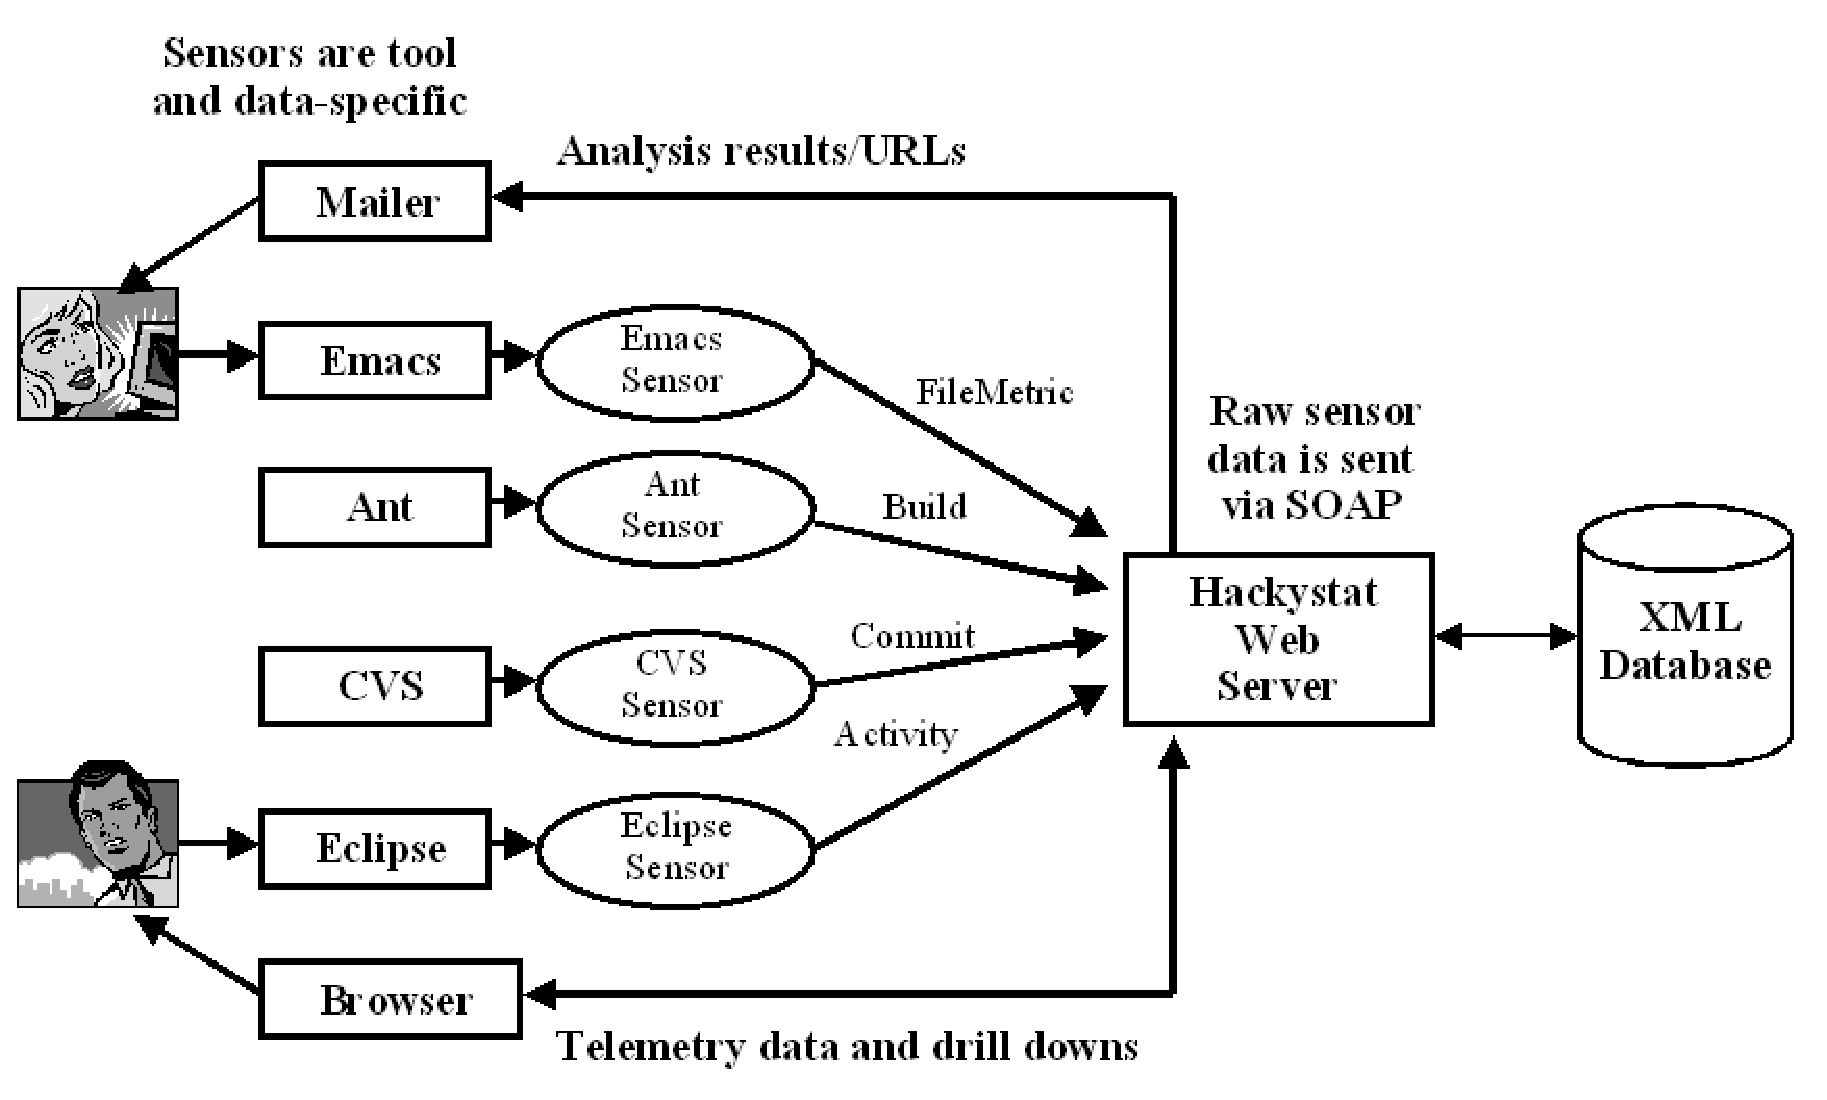
\includegraphics[width=0.60\textwidth]{architecture.eps}
%  \caption{The basic architecture of Hackystat. Sensors are attached to
%  tools directly invoked by developers (such as Eclipse or Emacs) as
%  well as to tools implicitly manipulated by developers (such as CVS or 
%  an automated build process using Ant).}
%  \label{fig:architecture}
%\end{figure*}

To use Hackystat, the project development environment is 
instrumented by installing Hackystat sensors, which developers attach
to the various tools such as their editor, build system, configuration
management system, and so forth. Once installed, the Hackystat sensors
unobtrusively monitor development activities and send process and
product data to a centralized web service.  If a user is working
offline, sensor data is written to a local log file to be sent
when connectivity can be established with the centralized web service.
Project members can then log in to the web server to see the collected
raw data and run analyses that integrate and abstract the raw sensor
data streams into telemetry.  Hackystat also allows project members to
configure ``alerts`` that watch for specific conditions in the
sensor data stream and send email when these conditions occur.

Hackystat is an open source project with sources, binaries, and
documentation available at http://www.hackystat.org.  There is also a
public server available at http://hackystat.ics.hawaii.edu.  Hackystat has
been under development for approximately three years, and currently
consists of around 900 classes and 60,000 lines of code.  Sensors are
available for a variety of tools including Eclipse, Emacs, JBuilder,
Jupiter, Jira, Visual Studio, Ant, JUnit, JBlanket, CCCC, DependencyFinder,
Harvest, LOCC, Office, and CVS.  

\Section {Software Project Telemetry}
\label{sec:telemetry}

A major application of Hackystat has been the development of a new
approach to software measurement analysis called ``Software Project
Telemetry``. We define Software Project Telemetry as a style of
software engineering process and product collection and analysis which
satisfies the following properties:

{\em Software project telemetry data is collected automatically by tools
that unobtrusively monitor some form of state in the project development
environment.}  In other words, the software developers are working in a
``remote or inaccessable location`` from the perspective of metrics
collection activities. This contrasts with software metrics data that
requires human intervention or developer effort to collect, such as PSP/TSP
metrics \cite{Humphrey95}.
        
{\em Software project telemetry data consists of a stream of time-stamped
events, where the time-stamp is significant for analysis.}  Software
project telemetry data is thus focused on evolutionary processes in
development.  This contrasts, for example, with Cocomo \cite{Boehm81},
where the time at which the calibration data was collected about the
project is not significant.

{\em Software project telemetry data is continuously and immediately
available to both developers and managers.}  Telemetry data is not hidden
away in some obscure database guarded by the software quality improvement
group.  It is easily visible to all members of the project for
interpretation.

{\em Software project telemetry exhibits graceful degradation.}  While
complete telemetry data provides the best support for project management,
the analyses should not be brittle: they should still provide value even if
sensor data occasionally ``drops out`` during the project. Telemetry
collection and analysis should provide decision-making value even if these
activities start midway through a project.
         
{\em Software project telemetry is used for in-process monitoring, control,
and short-term prediction.} Telemetry analyses provide representations of
current project state and how it is changing at the time scales of days,
weeks, or months.  The simultaneous display of multiple project state
values and how they change over the same time periods allow opportunistic
analyses---the emergent knowledge that one state variable appears to
co-vary with another in the context of the current project.

Software Project Telemetry enables a more incremental, distributed,
visible, and experiential approach to project decision-making. It also
creates perspectives on system development that can provide new insight
into HPC development processes, as we illustrate in the case study below.


\Section{Process and Product measures for HPC utilizing Hackystat}
\label{sec:metrics}

The development of an HPC system from a software engineering perspective
raises many interesting questions.  How long does such a system take to
develop?  Do some components take longer to develop than others?  How much
of the system is devoted to the sequential code, and how much is devoted
to the parallelization of this code?  How did the developer allocate their
time during development to these activities?  Do different choices of HPC
tools and technologies lead to different answers to these questions?  Would 
a different application area lead to similar or different results? 

We believe that automated infrastructure for the collection and
analysis of product and process data is an important first step toward
enabling the HPC community to generate answers to these questions,
and then use these answers to improve the tools and techniques for
HPC development.  The question is, what process and product measures
can be both automatically collected and used to provide interesting
insight into the questions raise above?  This case study investigates
the use of the following measures: Active Time, Most Active File,
Command Line Invocations, Parallel and Serial Lines of Code, Milestone
Test Success, and Performance.

The following sections describe each of these measures and illustrate them
with sample data from a one week ``snapshot'' of development of the Optimal
Truss Design problem in our case study. 

\SubSection{The Optimal Truss Design problem}
\label{sec:truss}

Our case study focuses on the development of a system for optimal truss
design.  Specifically, the system finds a pin-connected steel truss
structure that uses as little mass as possible to support a load connected
from three attachment points on a wall to the load-bearing point away from
the wall.  This problem was originally developed for use in research on
Purpose-Based Benchmarks (PBBs) \cite{Gustafson04}.  PBBs gather a
different and complementary set of metrics in order to assess productivity
in terms of acceptability to the customer.  

The system is being implemented by one of the authors, Michael Paulding, and
thus generally conforms to the ``lone researcher'' workflow for HPC development.  The
system development process and associated case study started in the Spring
of 2004 and is still ongoing.  To date, the implementation of the Optimal
Truss Design problem consists of approximately 1,200 source lines of code.

The solution to the Optimal Truss Design problem developed in this case
study involves several components. The first component is termed the
``sequential workhorse'', which includes the task of solving a truss once
all of its elements are defined.  Solving a truss includes the calculation
of its mass, which is determined by summing the mass of each of its
components (e.g. all steel joints and members).  In addition to mass
calculation, solving a truss also includes verifying equilibrium and
deformational constraints.  Equilibrium constraints require that all forces
and moments within a truss net zero magnitude, thus ensuring that the truss
is not accelerating.  Deformational constraints require that the length of
members (strut or cable) used in the truss do not exceed construction
safety limits.  These limits are defined and known prior to runtime.

\begin{figure}[htpb]
  \centering
  
\includegraphics[width=0.2\textwidth]{simple.truss.eps}
  \caption{An unoptimized solution to the Truss problem}
  \label{fig:simple_truss}
\end{figure}

\begin{figure}[htpb]
  \centering
  \includegraphics[width=0.2\textwidth]{multijoint.truss.eps}
  \caption{An optimized solution to the Truss problem}
  \label{fig:multijoint_truss}
\end{figure}

The second component of the Optimal Truss system generates the permutation
of all possible truss topologies within the domain space, ensuring that the
configuration with minimal mass is a global minimum.  The domain space for
the initial implementation is a 2-dimensional mesh of points, defining the
rectangle formed between the attachment points and the load bearing point.
Exploring all possible configurations results in a combinatorial explosion
as the mesh size is increased and this served as the first point of
parallelism in the implementation.  The task of parallelizing topology
generation can be equally divided among the available nodes.  This can be
accomplished in an ``embarrassingly parallel'' manner, where each row of
the mesh is assigned to a different processor to permute.

The third component of the system performs geometry assignment for all
trusses.  After generation, a topology defines the path of each truss from
the attachment points to the load bearing point, but it does not specify
what type of member connects each joint.  In this stage, either a strut or
a cable is substituted for each member, flushing out all permutations.
Once the geometry has been assigned, it can be given to a processor to
compute the mass of the truss and to determine whether the topology is
valid under the equilibrium and deformational constraints.

Now that the description of the Optimal Truss Design problem, used in our case study, has been explained, it is prudent to illustrate and investigate the measures applied to the problem.

\SubSection{Active Time}
\label{sec:activetime}

Active Time is a measure of the time spent by developers editing source
code (or other files) related to the system.  Active Time can be collected
automatically through the use of sensors attached to the editor used by
developers.  The sensors collect active time via a timer-based process
inside the editor that wakes up every 30 seconds and checks to see if the
active buffer has changed in identity or size since the last 30 seconds. If
so, a timestamped ``statechange" event is sent to the Hackystat server.
Active Time does not reflect effort spent by developers on the project that
does not involve editing files, including time spent viewing a file without
performing editing actions. Support for non-editing activities such as
``reading'' is a subject of future research, but even the restricted definition
of Active Time appears useful
in the HPC context as a proxy for overall effort.  For example, it helps a
development team answer questions such as: {\em ``How much of the overall
development effort was spent editing files?''} or {\em ``Did all team
members devote equal time to writing code?''} or {\em ``When was team effort 
focussed on code development during the project?''}

Figure \ref{fig:activetime} shows the Active Time associated with development of the
Optimal Truss Design application for a sample period in May, 2004.

\begin{figure*}[htpb]
  \centering
  \includegraphics[width=0.60\textwidth]{truss.activetime2.eps}
  \caption{Active time}
  \label{fig:activetime}
\end{figure*}

\SubSection{Most Active File}
\label{sec:mostactivefile}

A measure related to Active Time is the ``Most Active File".  One way to
abstract the raw event stream sent from an editor-based Hackystat server
begins by representing each day as a sequence of 288 five minute intervals.
If a developer actively edits one or more files within a five minute
period, then determine which file was edited most during that five minutes,
and assign the ``credit" for that five minute interval to that file and that
file alone, which we call the ``Most Active File''.  (We performed a
calibration study which found this to be a reasonable abstraction.)  The
Most Active File abstraction may be useful in the HPC context as a way of
determining what specific files were the focus of developer attention, and
how that focus of attention changed over the course of development.

For example, Figure \ref{fig:mostactivefile} shows the Most Active
Files associated with Optimal Truss Design during the first few days
of this time interval.  

\begin{figure*}[htpb]
  \centering
  \includegraphics[width=0.70\textwidth]{truss.mostactivefile.eps}
  \caption{Most Active File}
  \label{fig:mostactivefile}
\end{figure*}

\SubSection{Command Line Invocations}

In addition to time spent editing files in an editor, HPC development
frequently involves extensive use of shell processes to invoke programs
such as make, gcc, etc.  We have implemented a sensor for the Unix command
shell (based upon the 'history' shell mechanism) to record these command
line invocations. Command Line Invocation data can be useful in the HPC
context as a way of providing further insight into the types of activities
performed by developers during the development of the HPC code.  For
example, if the HPC developer spends significant time working at the
command line without concurrent editing of code, then it might be useful to
develop an enhanced representation of Active Time that accounts for this
type of effort as well. While the current sensor only captures command
invocations and not their results, it might be useful to extend the sensor
to capture the results of command line invocations in certain
circumstances. For example, recording whether or not a compilation
succeeded or failed as well as what types of run-time errors occur could
help identify potential development bottlenecks.

Figure \ref{fig:commandlineinvocations} illustrates Command Line Invocation data for 
a portion of one day during the  development of the Optimal Truss Design system.

\begin{figure*}[htpb]
  \centering
  \includegraphics[width=0.70\textwidth]{truss.commandlineinvocations.eps}
  \caption{Command Line Invocations}
  \label{fig:commandlineinvocations}
\end{figure*}

\SubSection{Parallel and Serial Size}

To understand HPC software development, it helps to be able to represent
both ``serial'' and ``parallel'' code.  We have enhanced our size
measurement tool, LOCC, with a token-based counter for C++ that allows us
to count non-comment source lines of code, and determine for each line of
code whether or not an MPI directive occurs on it.  Thus, for HPC programs
built using C++ and MPI, we can determine (a) the total number of files in
the system, (b) the total non-commented size of each file in the system;
(c) whether or not a file consists purely of serial (non-MPI) code or not;
(d) for files containing MPI directives, the frequency of occurrence of
each MPI directive; and (e) for files containing MPI code, what percentage
of the non-comment source lines of code contained an MPI directive.

Figures \ref{fig:parallelconstructs}, \ref{fig:parallelfiles},
and \ref{fig:parallelvsequential} provide perspectives on
size data for the Optimal Truss Design system.

\begin{figure*}[htpb]
  \centering
  \includegraphics[width=0.60\textwidth]{truss.parallelconstructs.eps}
  \caption{Parallel vs. sequential constructs}
  \label{fig:parallelconstructs}
\end{figure*}

\begin{figure*}[htpb]
  \centering
  \includegraphics[width=0.60\textwidth]{truss.parallelfiles.eps}
  \caption{Parallel vs. Sequential Files}
  \label{fig:parallelfiles}
\end{figure*}

\begin{figure*}[htpb]
  \centering
  \includegraphics[width=0.60\textwidth]{truss.parallelvsequential.eps}
  \caption{Parallel vs. Sequential SLOC}
  \label{fig:parallelvsequential}
\end{figure*}

\SubSection{Functionality}

We have defined a process for measuring the functionality of an HPC
application and tracking its development progress through the use of unit
testing.  We have termed this approach ``Progress Assessment through
Milestone Tests'' (PAMT).

Essentially, PAMT is a process in which HPC application designers draft
the specification for the system as a set of unit tests prior to
development.  Each unit test is defined such that it represents a
milestone, or significant aspect of application functionality.
Quantitative interpretation of ``significant'' is determined by the
application designer or program manager and is expected to vary between
HPC projects.  Defining the set of milestone tests prior to development
provides a specification for the system and also serves as a mechanism to
promote test driven design.

Once the milestone tests have been defined, the development team has a
concrete set of tests to implement that, together, represent the
functionality of the entire system.  The development team can then
implement the milestone tests in any order and their progress through
the application can be monitored.  System progress and functionality
is measured by investigating the number of milestone tests passing in
ratio to the total number of milestone tests representing the system.
In most cases, a development team will begin implementation with zero
milestone tests passing and finish development when all milestone
tests pass.

For the Optimal Truss Design problem, a set of 10 milestone tests were
defined prior to implementation.  Individually, each test represents a
significant functionality of the application and together they provide a
specification for the entire system.  For the Optimal Truss problem, the
milestone tests were written in CppUnit, a unit test framework for the C++
programming language.  Below is an example of a single milestone test for
the Optimal Truss problem.

\begin{quotation}
\noindent {\bf Milestone Test 4:} This test verifies that the application is 
capable of representing a 2-dimensional topology.  In the Optimal Truss
specification, a topology is defined as a set of 2 trusses that
individually connect the 2 attachment points to the load bearing
point.  Interconnections (members) between the trusses are allowed.
Therefore, for this milestone test, given 2 attachment points, a load
bearing point and the number of joints, the application must be able
to query:

\begin{enumerate}
\item Each of the trusses connecting the 2 attachment points to the load
bearing point
\item The set of members composing one of the trusses in the topology
\item Given a truss, whether it is part of the topology
\end{enumerate}
\end{quotation}

\begin{figure*}[htpb]
  \centering
  \includegraphics[width=0.60\textwidth]{truss.functionality.eps}
  \caption{Progress Assessment through Milestone Tests}
  \label{fig:functionality}
\end{figure*}

From this chart is is evident that during the development period from
04-May-2004 through 11-May-2004 that the Optimal Truss application
progressed from 1 milestone test passing at the beginning of the
interval to 5 milestone tests passing at the end.  It is important to
note that this interval represents a sample of the development period
and does not capture start to finish.  In addition, this trend
indicates a consistent increase in passing milestone tests.  However,
it is quite possible for development to lower the number of successful
milestone tests, indicated by a negative slope in the trend.

\SubSection{Performance}

The high performance computing community has developed a broad range of
standard measures to characterize parallel performance, including degree of
parallelism, average parallelism, speedup, redundancy, and utilization.
In this research, we are not attempting to specify the ``right'' performance
measure for any particular application area. Instead, we advocate that 
performance be measured regularly throughout development using as many metrics
as necessary to best characterize the application. 

Performance measures are not generally interesting as absolute numbers,
since the absolute values are obviously dependent upon current hardware and
other physical resources. Performance measures are interesting as relative
numbers, in the sense that the way they change over time tells us whether
or not and to what extent developers could tune an initial implementation
to improve its performance, how the code evolved to obtain this performance
increase, and whether or not functionality was sacrificed in order to do
so.

Figure \ref{fig:performance} shows the execution (wall time) performance of the 
Optimal Truss Design system developed in the case study for a sample time interval. 

\begin{figure*}[htpb]
  \centering
  \includegraphics[width=0.60\textwidth]{truss.performance.eps}
  \caption{Truss Execution Time Performance}
  \label{fig:performance}
\end{figure*}


\Section{Conclusions}
\label{sec:conclusions}

After accumulating the data trends provided by the Hackystat system,
we are able to gain insights that assist in understanding the
development of HPC applications.  From the graphs presented earlier,
we are able to make interpretations about development activities,
development progress and application performance and functionality
tradeoffs.

\SubSection{Development Activities}
\label{sec:devactivities}

From the data presented in Figure \ref{fig:commandlineinvocations} we
are able to interpret the developer activities of that particular day.
The daily dairy for 06-May-2004 lists all the commands issued to the
console on that day.  Figure \ref{fig:commandlineinvocations} is a
sample of all the command line invocations issued, but it provides
insight to the developer activities on that day.

For example, from the command line invocations and most active file
data for 06-May-2004, we can observe that the developer devoted the
most time on the {\it test\_distribution.cc} file.  It so happens that this
file implements the distribution of 2-dimensional mesh from which the
truss topologies are constructed.  Furthermore, the distribution of
topologies is a significant function of the Optimal Truss problem and
has been designated as a milestone test of the system.  Therefore,
from this data, an observer can conclude that the developer was
investing his efforts on implementing functionality on this day,
rather than on increasing performance by optimizing code.

In addition, an observer, such as a project manager or the developer
himself, can observe the active time trend in Figure
\ref{fig:activetime} to understand the time invested to implement a
particular milestone.  For example, in Figure \ref{fig:activetime} on
06-May-2004, it is evident that the developer spent over 5 hours
editing code to implement the topology distribution milestone.

\SubSection{Development Progress}
\label{sec:devprogress}

The data presented in Progress Assessment through Milestone Tests (PAMT)
chart, as illustrated in Figure \ref{fig:functionality}, provides a clear illustration
of the real-time progress being made on the Optimal Truss problem.

There are two trends presented in this figure, one representing the
total number of milestone tests defined for the Optimal Truss problem
and the other representing the number of milestone tests passing at
the conclusion of each day.  

In the Optimal Truss problem, the total milestone tests are
represented by the horizontal line fixed at 10 unit tests.  This
indicates that there are 10 milestone tests encompassing the Optimal
Truss problem and that the project manager has not added or removed
any of these milestones during this time interval.  It is quite
possible that a project manager may have to alter milestones in order
to meet deadlines and this analysis provides a trend for this purpose.
For example, if the total milestone tests is altered, the total tests
trend on the chart will move up or down accordingly.

The PAMT chart also allows an observer to track the progress made
through the application.  For example, in this figure, the lower trend
represents the number of milestone tests passing on each day.  Every
time a new milestone test passes, it indicates that another unit of
functionality has been added to the system provided that all
previously passing tests still pass after the change.

Coupling the PAMT data with the active time data in Figure
\ref{fig:activetime}, an observer is also able to interpret a
quantitative measurement of how much development time was devoted to a
particular unit of functionality.  For example, on 06-May-2004,
approximately 5 hours of editing were invested to add one unit of
functionality to the application.  This is indicated by the number of
passing milestone tests increasing from one to two on this day.  In
addition, an observer can quickly understand the percentage complete
of the system.  On 06-May-2004, the Optimal Truss problem has 2 out of
10 milestone tests passing and is therefore 20\% complete.

\SubSection{Application Performance and Functionality Tradeoffs}
\label{sec:appperfvsfunctionality}

When one combines the data presented in the Performance chart in Figure
\ref{fig:performance} with the PAMT Functionality chart in Figure
\ref{fig:functionality}, it reveals an example of the 
interactions between performance and functionality in HPC development.

One of the primary objectives of HPC development is to obtain the
fastest possible execution time of the system.  This goal influences
developers to frequently (if not constantly) think about or perform
optimization on their code.

However, as functionality is added to the application, it is common
for the performance of the system to decrease, indicated by an
increase in execution time.

The data presented in figures \ref{fig:performance} and
\ref{fig:functionality} reveal this
performance and functionality tradeoff.  For example, execution time
between 04-May-2004 and 07-May-2004 increaseses roughly from 30.0
hours to 32.5 hours.  On the other hand, 3 additional milestone tests,
representing system functionality, are implemented successfully during
this interval.  This indicates that three units of functionality have been
added at the cost of an addition of approximately 10\% in execution time.

Data presented in these figures allow project managers to understand
how functionality increases affect system performance.  It also gives
them a starting point to determine which functionality should be
optimized in the case where the performance degradation is not
acceptable.  Trends such as these enable project managers and
developers to understand the development process and make in-process
decisions to affect the development outcome.

In conclusion, we have found that Active Time, Most Active File, Command
Line Invocations, Parallel and Serial Lines of Code, Milestone Test
Success, and Performance constitute an interesting set of process and
product measures that can be automatically collected during HPC
development.  As our case study continues, we will look for other
opportunities to use this measures to gain insight into opportunities to
improve high performance computing.

\Section{Acknowledgements}
\label{sec:acknowledgements}
We would like to thank the University of Hawaii and MHPCC (Maui High Performance Computing Center) for their continued support of and interest in our research.
 
\bibliographystyle{/export/home/csdl/tex/icse2003/latex8}
\bibliography{/export/home/csdl/techreports/04-11/04-11,/export/home/csdl/bib/csdl-trs,/export/home/csdl/bib/hackystat,/export/home/csdl/bib/psp,/export/home/csdl/bib/hpcs}
\end{document}
 










